\section{Auswertung}
\label{sec:Auswertung}

\subsection{Untersuchung der Phasenabhängigkeit der Ausgangsspannung}
\label{sec:Untersuchung der Phasenabhängigkeit der Ausgangsspannung}
Im ersten Teil wurde der Zusammenhang zwischen Ausgangsspannung und der Phase der
Referenzspannung untersucht. Dabei wurden sieben Messwerte aufgenommen, welche in
\autoref{fig:plot-phase} dargestellt sind. Die Messdaten sind zusätzlich auch in 
\autoref{tab:messdaten-phase} abgedruckt.
\begin{table}[H]
	\centering
	\caption{Messergebnisse zur Lichtintensität der LED.}
	\label{tab:messdaten-phase}
	\sisetup{table-format=2.1}
	\begin{tabular}{c c c}
		\toprule
		$\phi / \si{\deg}$ & $\phi / \si{rad}$ & $U / \si{\volt}$ \\
		\midrule
		0	& $0$			&38  \\
		60	& $\frac\pi3$		&27 \\
		120	& $\frac{2\pi}3$	&27 \\
		180	& $\pi$			&-38 \\
		240	& $\frac{4\pi}3$	&-28 \\
		300	& $\frac{5\pi}3$	&-28 \\
		360	& $2\pi$		&38 \\
		\bottomrule
	\end{tabular}
\end{table}
\begin{figure}
	\centering
	\includegraphics{phase.pdf}
	\caption{Messdaten und Curve Fit für den Zusammenhang zwischen Ausgangsspannung und
	Phase der Referenzspannung. In rot ist zusätzlich die in \autoref{sec:Theorie}
	errechnete Theoriekurve $U(\phi) \propto \cos(\phi)$ gezeichnet.}
	\label{fig:plot-phase}
\end{figure}
Die Amplitude wird durch einen Cosinus beschrieben. Daher liegt eine Fitfunktion der Form
\begin{equation}
	U(\phi) = a \cdot \sin\left(b \cdot \phi + c\right) + d
\end{equation}
nahe.
Der Curve Fit aus scipy hat dabei die Parameter
\begin{equation}
	a = (42,3 \pm 10,2) \, \si{\volt}
	\quad
	b = (0,96 \pm 0,12)
	\quad
	c = (0,86 \pm 0,49)
	\quad
	d = (2 \pm 7,8) \, \si{\volt}
	\label{eqn:parameter-phase}
\end{equation}
errechnet

\subsection{Untersuchung der Auswirkung des Noise Generators}
\label{sec:Untersuchung der Auswirkung des Noise Generators}
Neben den quantitativen Untersuchungen wurde auch der Effekt des Noise Generators
untersucht. Dabei sind die zwei Aufnahmen jeweils mit und ohne Noise Generator in 
\autoref{fig:noise-gen} abgebildet.
\begin{figure}[H]
	\centering
	\begin{subfigure}[b]{0.45\textwidth}
		\centering
		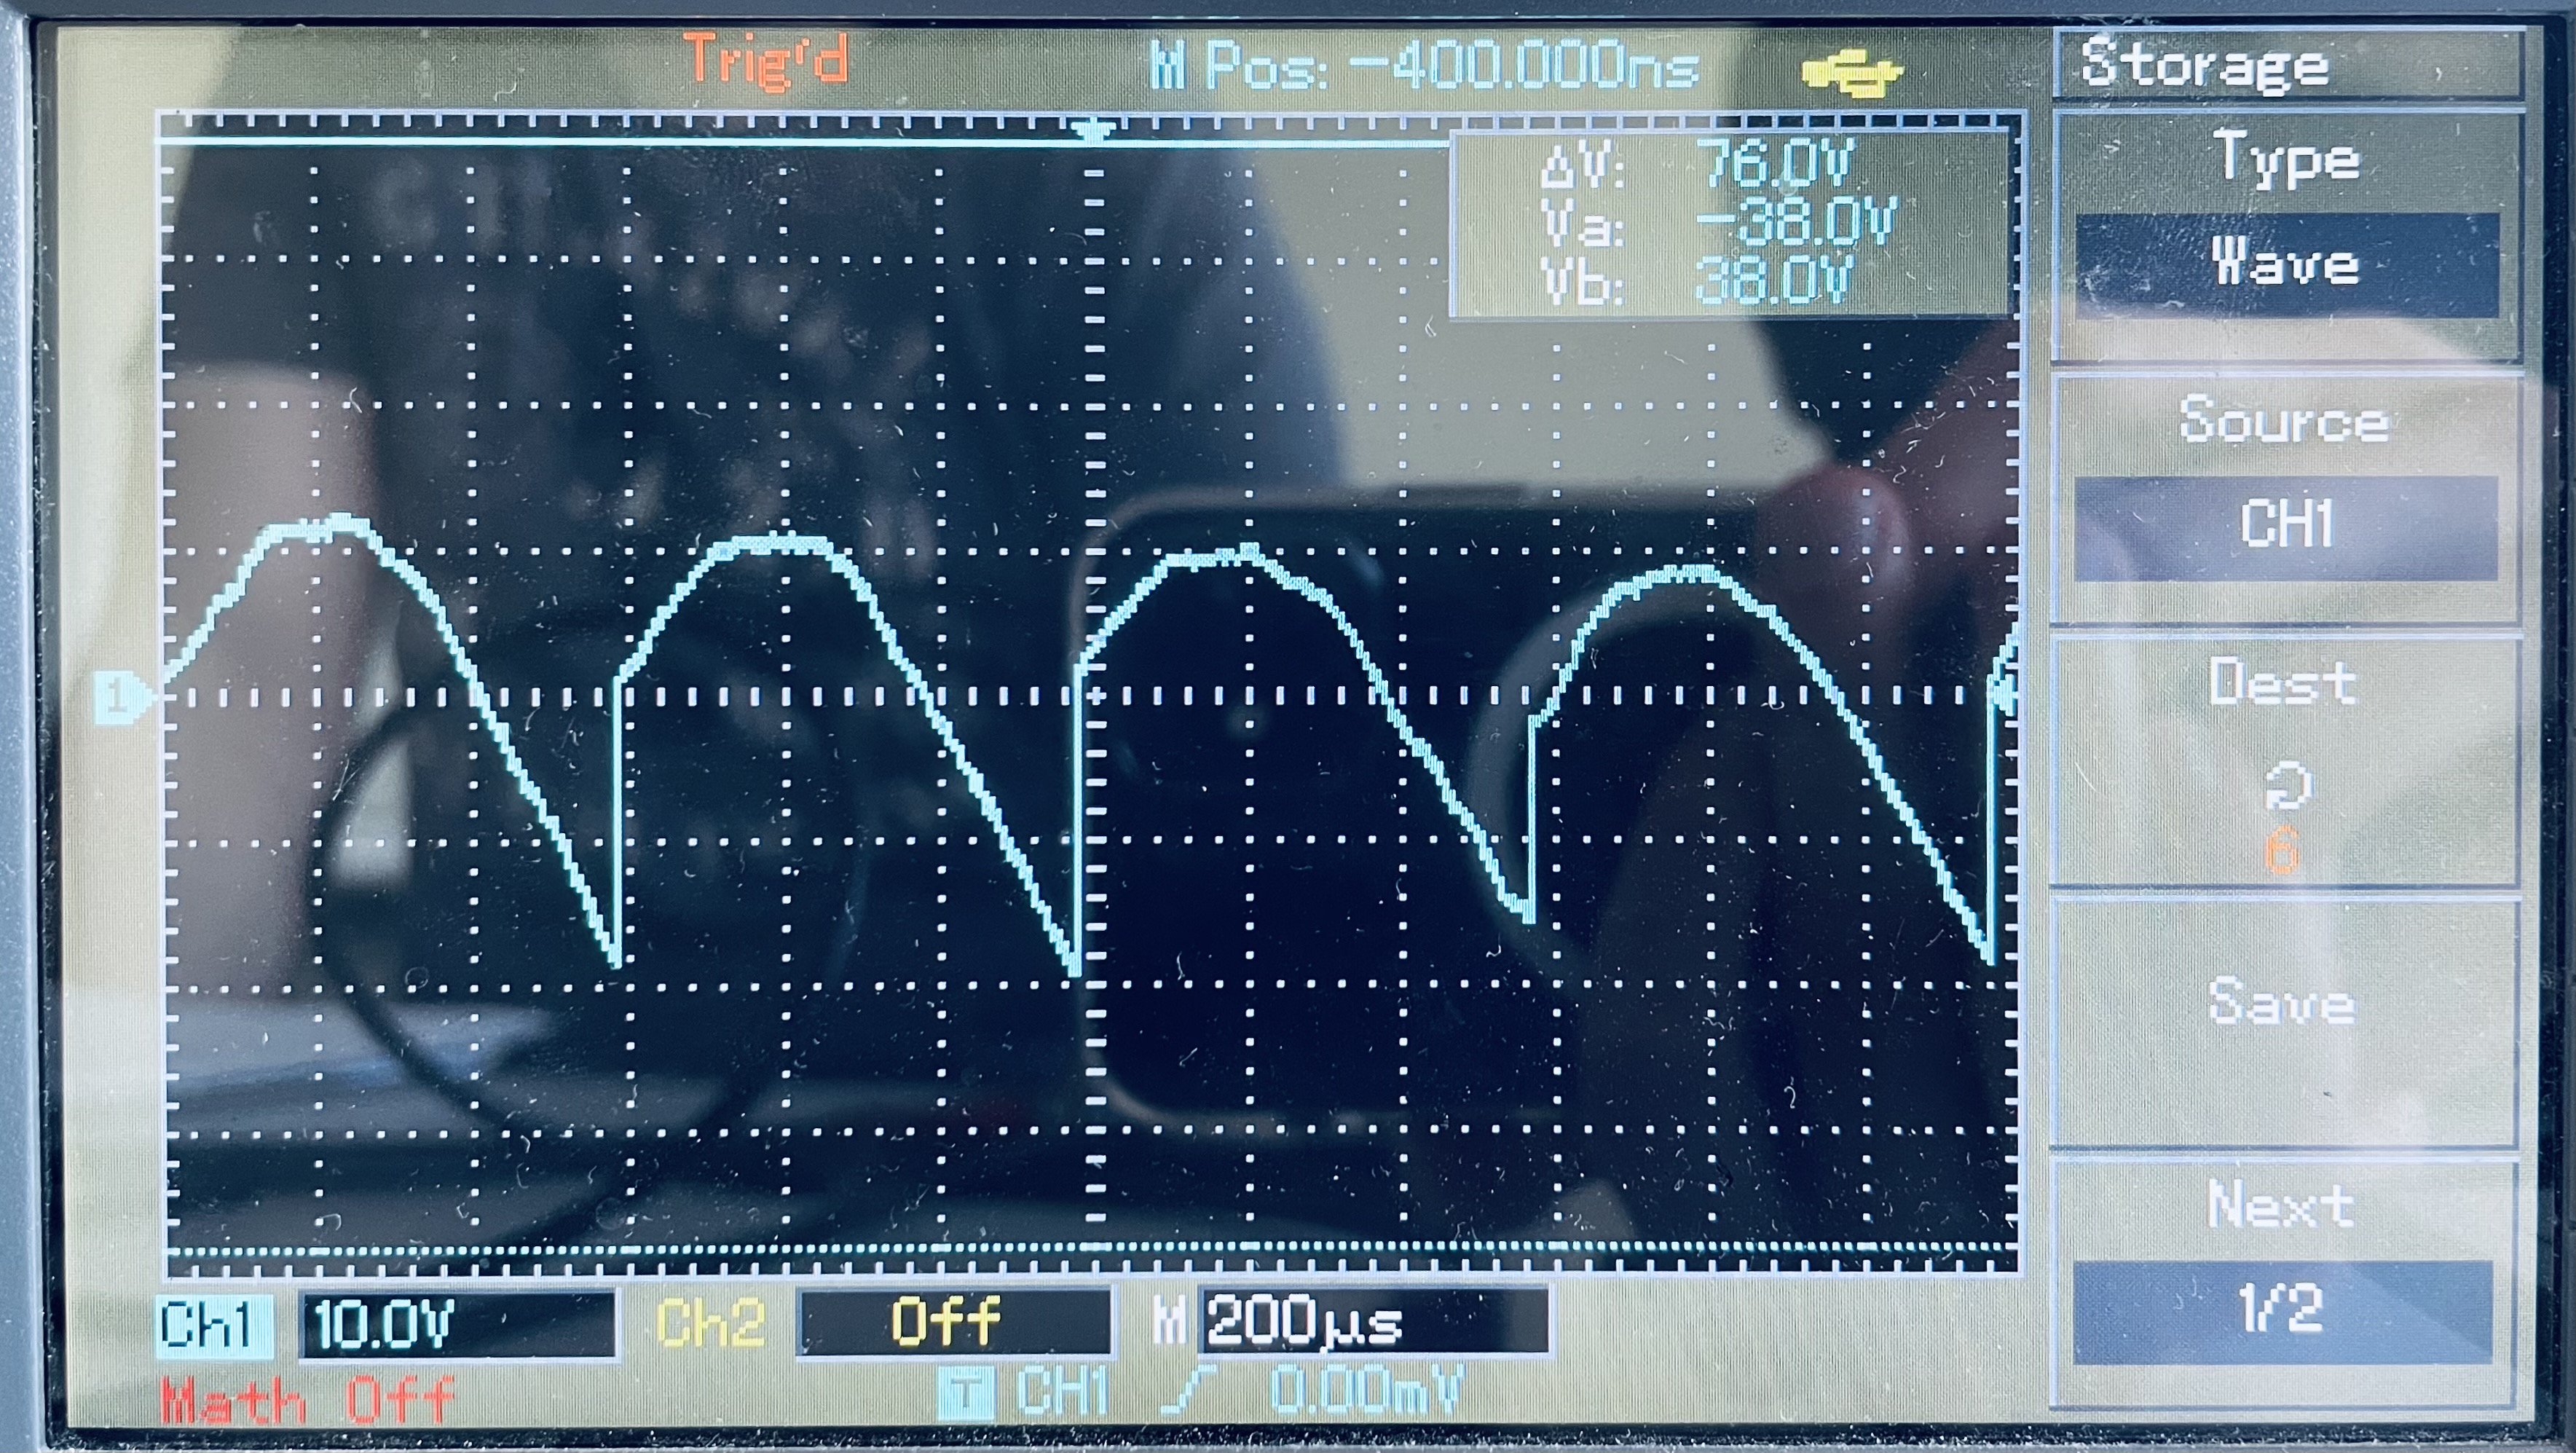
\includegraphics[width=\textwidth]{images/no-noise.JPG}
		\caption{Oszillographenaufnahme ohne Rauschgenerator.}
		\label{fig:osc-no-noise}
	\end{subfigure}
	\hfill
	\begin{subfigure}[b]{0.45\textwidth}
		\centering
		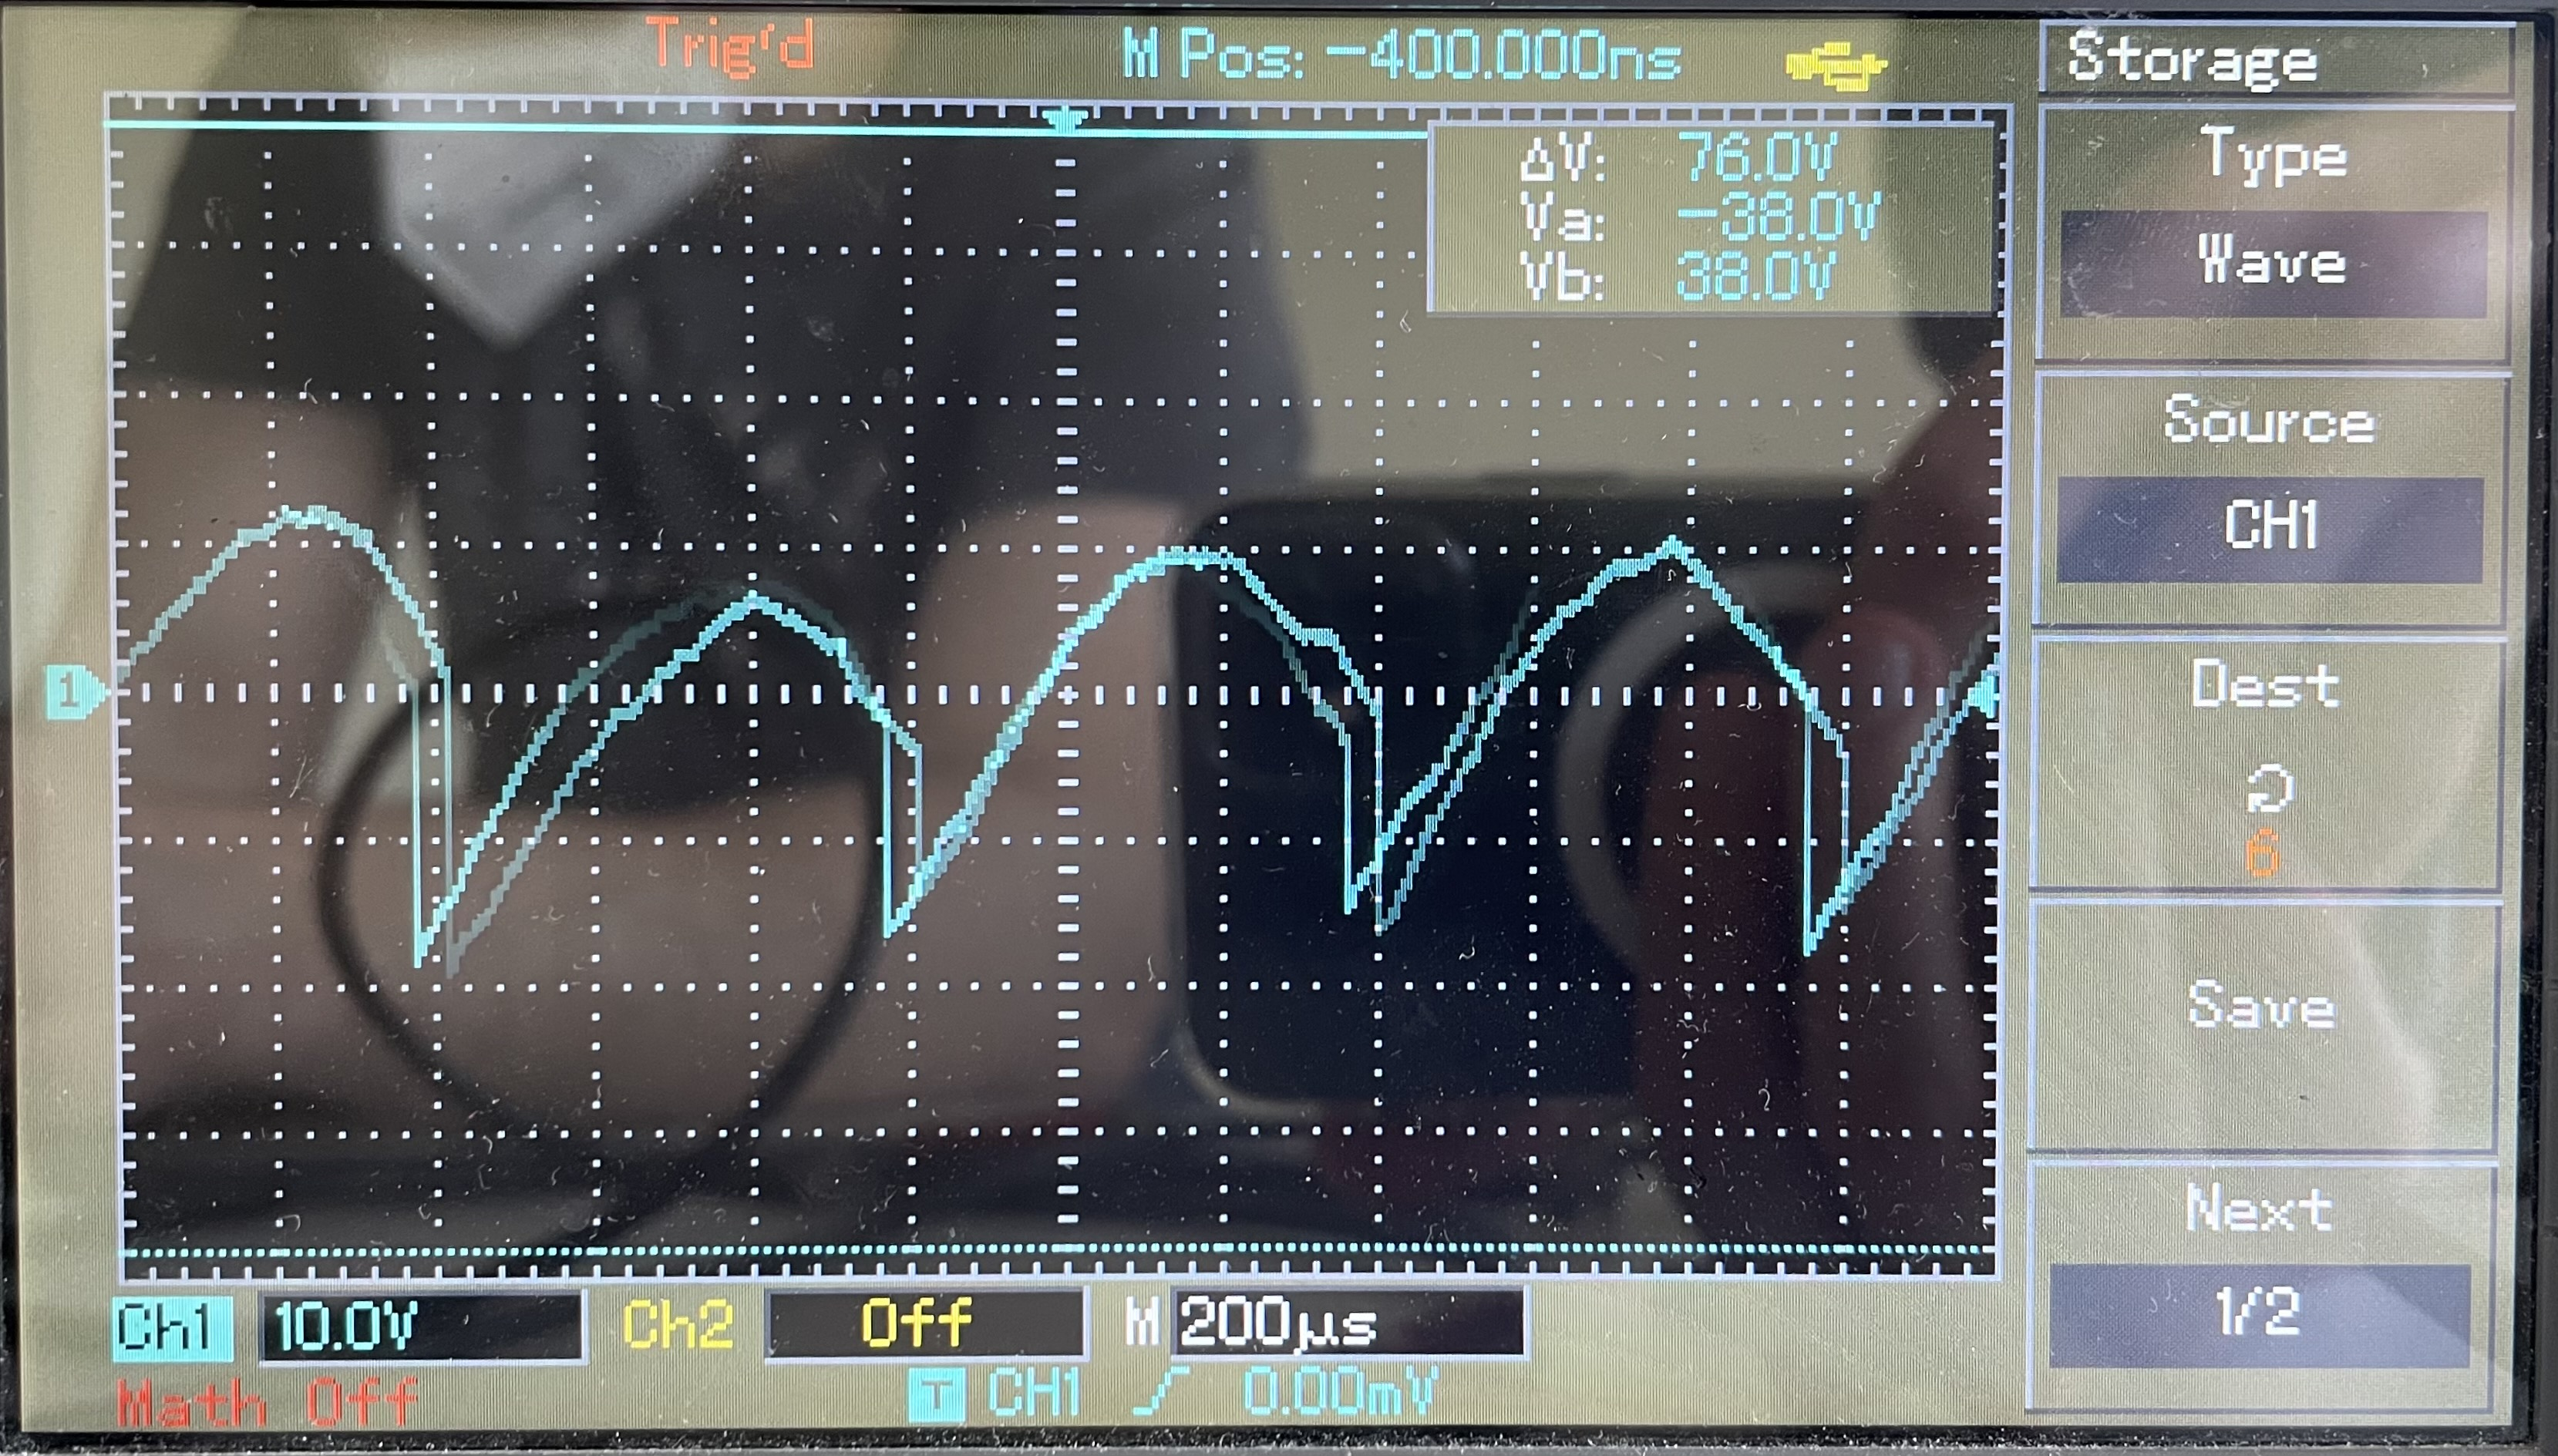
\includegraphics[width=\textwidth]{images/noise.jpg}
		\caption{Oszillographenaufnahme mit Rauschen.}
		\label{fig:osc-noise}
	\end{subfigure}
	\caption{Aufnahmen mit und ohne Rauschengenerator.}
	\label{fig:noise-gen}
\end{figure}

\subsection{Messung der Lichtintensität einer LED}
\label{sec:Messung der Lichtintensität einer LED}
Mit der in \autoref{sec:Durchführung} beschriebenen Apparatur wurden die in 
\autoref{tab:messdaten-led} gedruckten Messdaten aufgenommen. 
Aufgrund der Ausbreitung der Lichtwellen wird
hier eine Fitfunktion der Form
\begin{equation}
	f(d) = \frac{a}{d} + b
\end{equation}
verwendet.\\
Der Curve Fit hat hier die Parameter
\begin{equation}
	a = (637 \pm 51,2) \, \frac{\si{\volt}}{\si{\centi\meter}}
	\qquad
	b = (-20,7 \pm 3,5) \, \si{\volt}
\end{equation}
gefunden. Zusätzlich wurde ein alternativer Fit mit einem $1 / x^2$ Abfall durchgeführt.
Die Fitfunktion
\begin{equation}
	g(d) = \frac{a^\prime}{d^2} + b^\prime
\end{equation}
wurde dabei mit den Paramtern
\begin{equation}
	a^\prime = (4988 \pm 147,4) \, \frac{\si{\volt}}{\si{\centi\meter}}
	\qquad
	b^\prime = (-3 \pm 0,82) \, \si{\volt}
\end{equation}
angepasst.
\begin{table}
	\centering
	\caption{Messergebnisse zur Lichtintensität der LED.}
	\label{tab:messdaten-led}
	\sisetup{table-format=2.1}
	\begin{tabular}{c c}
		\toprule
		$d / (\si{\centi\meter})$ & $U / \si{\volt}$ \\
		\midrule
		9,55         &           54 \\
		11           &           38 \\
		12           &           30 \\
		13           &           26 \\
		14           &           20 \\
		15           &           18 \\
		17           &           16 \\
		20           &           10 \\
		25           &           5  \\
		30           &           3  \\
		35           &           2  \\
		\bottomrule
	\end{tabular}
\end{table}
Die Messdaten sowie Ausgleichskurve sind in \autoref{fig:plot-diode} dargestellt.
\begin{figure}
	\centering
	\includegraphics{diode.pdf}
	\caption{Messdaten und Curve Fit der Lichtintensität in Abhängigkeit von der
	Distanz.}
	\label{fig:plot-diode}
\end{figure}
